\documentclass[a4paper,12pt]{article}

\usepackage{float}


\usepackage[utf8]{inputenc}
\usepackage[dvips]{graphicx}
%\usepackage{a4wide}
\usepackage{epsfig}
\usepackage{fancybox}
\usepackage{verbatim}
\usepackage{array}
\usepackage{latexsym}
\usepackage{alltt}
\usepackage{amssymb}
\usepackage{amsmath,amsthm}
\usepackage{bm}
\usepackage{wasysym}

%\usepackage{fullpage}
%\usepackage{hyperref}
\usepackage{listings}
\usepackage{color}
\usepackage{algorithm}
\usepackage{algpseudocode}
\usepackage[hmargin=2cm,vmargin=3.0cm]{geometry}
%\topmargin=0cm
%\topmargin=-1.8cm
%\addtolength{\textheight}{6.5cm}
%\addtolength{\textwidth}{2.0cm}
%\setlength{\leftmargin}{-3cm}
%\setlength{\oddsidemargin}{0.0cm}
%\setlength{\evensidemargin}{0.0cm}

%misc libraries goes here
\usepackage{tikz}
\usepackage{tikz-qtree}
\usetikzlibrary{automata,positioning}

\usepackage{multicol}
\usepackage{enumitem}

\usepackage[most]{tcolorbox}

\usepackage[colorlinks=true,urlcolor=black,linkcolor=black]{hyperref}


\lstdefinestyle{customtex}{
    %backgroundcolor=\color{lbcolor},
    tabsize=2,
    language=TeX,
    numbers=none,
    basicstyle=\footnotesize\ttfamily,
    numberstyle=\footnotesize,
    aboveskip={0.0\baselineskip},
    belowskip={0.0\baselineskip},
    %
    columns=flexible,
    keepspaces=true,
    fontadjust=true,
    upquote=true,
    %
    breaklines=true,
    prebreak=\raisebox{0ex}[0ex][0ex]{\ensuremath{\hookleftarrow}},
    frame=single,
    showtabs=false,
    showspaces=false,
    showstringspaces=false,
    %
    %identifierstyle=\color[rgb]{0,0.2,0.8},
    identifierstyle=\color[rgb]{0,0,0.5},
    %identifierstyle=\color[rgb]{0.133,0.545,0.133},
    %keywordstyle=\color[rgb]{0.8,0,0},
    %keywordstyle=\color[rgb]{0.133,0.545,0.133},
    keywordstyle=\color[rgb]{0,0,0.5},
    %commentstyle=\color[rgb]{0.133,0.545,0.133},
    commentstyle=\color[rgb]{0.545,0.545,0.545},
    %stringstyle=\color[rgb]{0.827,0.627,0.133},
    stringstyle=\color[rgb]{0.133,0.545,0.133},
    %
    literate={â}{{\^{a}}}1 {Â}{{\^{A}}}1 {ç}{{\c{c}}}1 {Ç}{{\c{C}}}1 {ğ}{{\u{g}}}1 {Ğ}{{\u{G}}}1 {ı}{{\i}}1 {İ}{{\.{I}}}1   {ö}{{\"o}}1 {Ö}{{\"O}}1 {ş}{{\c{s}}}1 {Ş}{{\c{S}}}1 {ü}{{\"u}}1 {Ü}{{\"U}}1 {~}{$\sim$}{1}
}

\lstdefinestyle{output}{
    %backgroundcolor=\color{lbcolor},
    tabsize=2,
    numbers=none,
    basicstyle=\footnotesize\ttfamily,
    numberstyle=\footnotesize,
    aboveskip={0.0\baselineskip},
    belowskip={0.0\baselineskip},
    %
    columns=flexible,
    keepspaces=true,
    fontadjust=true,
    upquote=true,
    %
    breaklines=true,
    prebreak=\raisebox{0ex}[0ex][0ex]{\ensuremath{\hookleftarrow}},
    frame=single,
    showtabs=false,
    showspaces=false,
    showstringspaces=false,
    %
    %identifierstyle=\color[rgb]{0.44,0.12,0.1},
    identifierstyle=\color[rgb]{0,0,0},
    keywordstyle=\color[rgb]{0,0,0},
    commentstyle=\color[rgb]{0,0,0},
    stringstyle=\color[rgb]{0,0,0},
    %
    literate={â}{{\^{a}}}1 {Â}{{\^{A}}}1 {ç}{{\c{c}}}1 {Ç}{{\c{C}}}1 {ğ}{{\u{g}}}1 {Ğ}{{\u{G}}}1 {ı}{{\i}}1 {İ}{{\.{I}}}1   {ö}{{\"o}}1 {Ö}{{\"O}}1 {ş}{{\c{s}}}1 {Ş}{{\c{S}}}1 {ü}{{\"u}}1 {Ü}{{\"U}}1
}

\lstset{style=customtex}


\tikzset{%
    terminal/.style={draw, rectangle,
    				 align=center, 
					 minimum height=1cm, 
					 minimum width=2cm,
					 fill=black!10,
					 anchor=mid},
    nonterminal/.style={draw, rectangle,
    					align=left,
					    minimum height=1cm, 
						minimum width=2cm, 
						anchor=mid},% and so on
}

%% Style for terminals
%\tikzstyle{terminal}=[draw, rectangle, 
%					  minimum height=1cm, 
%					  minimum width=2cm, 
%					  fill=black!20,
%					  anchor=south west]
%% Style for nonterminals
%\tikzstyle{nonterminal}=[draw, rectangle, 
%						 minimum height=1 cm, 
%						 minimum width=2 cm, 
%						 anchor=north east]


\newcommand{\HRule}{\rule{\linewidth}{1mm}}
\newcommand{\kutu}[2]{\framebox[#1mm]{\rule[-2mm]{0mm}{#2mm}}}
\newcommand{\gap}{ \\[1mm] }

\newcommand{\Q}{\raisebox{1.7pt}{$\scriptstyle\bigcirc$}}
\newcommand{\minus}{\scalebox{0.35}[1.0]{$-$}}

\setlength{\fboxsep}{10pt}

\tcbsetforeverylayer{enhanced jigsaw, breakable, arc=0mm, boxrule=1pt, boxsep=5pt, after=\vspace{1em}, colback=white, colframe=black}

\newcolumntype{P}[1]{>{\centering\arraybackslash}p{#1}}

\setlength\parindent{0pt}

%\renewcommand\arraystretch{1.2}

\newenvironment{Tab}[1]
  {\def\arraystretch{1}\tabular{#1}}
  {\endtabular}

%%%%%%%%%%%%%%%%%%%%%%%%%%%%%%%%%%%%%%%%%%%%%%%%%%%%%%%%%%%%%%%%%%%%%%%%%%%%%%%%%%%%%%

\title{CENG 352 - Database Management Systems \\ Written Assignment 1}
\author{Yavuz Selim YESILYURT \\ 2259166} % write your name and id
\date{05.04.2020}

%%%%%%%%%%%%%%%%%%%%%%%%%%%%%%%%%%%%%%%%%%%%%%%%%%%%%%%%%%%%%%%%%%%%%%%%%%%%%%%%%%%%%%

\begin{document}
\HRule\\
Middle East Technical University \hfill Department of Computer Engineering
{\let\newpage\relax\maketitle}
\HRule\\
\vspace{1cm}

%%%%%%%%%%%%%%%%%%%%%%%%%%%%%%%%%%%%%%%%%%%%%%%%%%%%%%%%%%%%%%%%%%%%%%%%%%%%%%%%%%%%%%

% Write your answers below the section tags
\section{E/R Diagram \hfill}

\paragraph{a)} Necessary SQL DDLs to resemble the E/R diagram are below:  \\  

\begin{tcolorbox}
CREATE TABLE Department ( \\ 
	dept\_id int, \\ 
	location varchar(50), \\ 
	name varchar(50),\\
	PRIMARY KEY (dept\_id));
\end{tcolorbox}

\begin{tcolorbox}
CREATE TABLE Employee ( \\
	emp\_id int, \\
	surname varchar(50), \\
	name varchar(50), \\
	salary int, \\
	gender varchar(50), \\
	PRIMARY KEY (emp\_id));
\end{tcolorbox}

\newpage

\begin{tcolorbox}
CREATE TABLE Reports\_to ( \\
	supervisor\_emp\_id int, \\
	subordinate\_emp\_id int, \\
	PRIMARY KEY (supervisor\_emp\_id, subordinate\_emp\_id), \\
  	FOREIGN KEY (supervisor\_emp\_id) REFERENCES Employee(emp\_id), \\
  	FOREIGN KEY (subordinate\_emp\_id) REFERENCES Employee(emp\_id));
\end{tcolorbox}

\begin{tcolorbox}
CREATE TABLE Works\_in ( \\
	dept\_id int not null, \\
	emp\_id int, \\
	PRIMARY KEY (dept\_id, emp\_id), \\
  	FOREIGN KEY (dept\_id) REFERENCES Department(dept\_id) ON DELETE NO ACTION, \\
  	FOREIGN KEY (emp\_id) REFERENCES Employee(emp\_id) ON DELETE CASCADE);
\end{tcolorbox}

\begin{tcolorbox}
CREATE TABLE Manages ( \\
	dept\_id int, \\
	emp\_id int not null DEFAULT 101, \\
	PRIMARY KEY (dept\_id), \\
  	FOREIGN KEY (dept\_id) REFERENCES Department(dept\_id), \\
  	FOREIGN KEY (emp\_id) REFERENCES Employee(emp\_id) ON DELETE SET DEFAULT);
\end{tcolorbox}

\begin{tcolorbox}
CREATE TABLE Runs\_Project ( \\
	dept\_id int, \\
	project\_id int, \\
	budget int, \\
	due\_date date, \\
	state varchar(50), \\
	PRIMARY KEY (dept\_id, project\_id), \\
  	FOREIGN KEY (dept\_id) REFERENCES Department(dept\_id));
\end{tcolorbox}

\newpage
\paragraph{b)} An assertion called Total to enforce the total participation constraint: \\

\begin{tcolorbox}
CREATE ASSERTION Total \\
CHECK (NOT EXISTS ( \\
                    SELECT emp\_id \\
                    FROM Employee \\
                    EXCEPT \\
                    SELECT DISTINCT emp\_id \\
                    FROM works\_in))
\end{tcolorbox}

\paragraph{c)} SQL CHECK clauses to implement the given constraints: \\

\begin{tcolorbox}
CHECK (Salary $>$ 3600)
\end{tcolorbox}

\begin{tcolorbox}
CHECK (name LIKE CONCAT('\%', location, '\%'))
\end{tcolorbox}

\paragraph{d)} An after trigger to implement the given constraint: \\

\begin{tcolorbox}
CREATE TRIGGER CheckBudgetOnChange \\
AFTER UPDATE OF budget ON Runs\_Project \\
REFERENCING \\
OLD ROW AS OldRow \\
NEW ROW AS NewRow \\
FOR EACH ROW \\
WHEN (OldRow.budget $>$ NewRow.budget) \\
UPDATE Runs\_Project
SET state = 'Unsuccessful' \\
WHERE Runs\_Project.dept\_id = OldRow.dept\_id AND \\
Runs\_Project.project\_id = OldRow.project\_id 
\end{tcolorbox}

\newpage
\section{Maximum Number of Tuples}

\paragraph{a)}Assume that the Product table consists of 100 rows with unique id’s, the Store table has 5 rows with unique id’s and the Person table contains 1000 rows with unique id’s. \\

\begin{tcolorbox}
We have the following definition of relation $R$ for the given E/R diagram:
\begin{center}
    R(\underline{prodId}, \underline{storeId}, personId)
\end{center}
We will have a distinct record for each unique primary key tuple, i.e. a distinct record for each unique "prodId" and "storeId" attributes. Since there are 100 unique products in Product table and 5 stores in Store table, we will have $100 * 5 = 500$ records in relation $R$ as a result.
\end{tcolorbox}

\paragraph{b)}Assume that the Product table consists of 100 rows with unique id’s, the Store table has 5 rows with unique id’s and among 1000 Person entries there are 10 SalesPerson. \\

\begin{tcolorbox}
We have the following definition of relation $R$ for the given E/R diagram:
\begin{center}
    R(\underline{prodId}, storeId, sales\_personId, \underline{customer\_personId})
\end{center}
We will have a distinct record for each unique primary key tuple, i.e. a distinct record for each unique "prodId" and "customer\_personId" attributes. Since there are 100 unique products in Product table and 990 customers in Person table, we will have $100 * 990 = 99000$ records in relation $R$ as a result.
\end{tcolorbox}

\section{Armstrong’s Axioms}

First let us enumerate the given functional dependencies to refer them later in the proofs. We have: \\
1) A $\rightarrow$ C \\
2) B $\rightarrow$ E \\
3) CB $\rightarrow$ F \\
4) FE $\rightarrow$ G \\
5) FG $\rightarrow$ AH \\

I am going to continue enumerating also my findings to be able to refer them later.

\paragraph{a)} let us prove CB $\rightarrow$ G by using Armstrong's Axioms \\

\begin{tcolorbox}
6) CB $\rightarrow$ B (Trivial) \\
7) CB $\rightarrow$ E (Transitivity on 2, 6) \\
8) CB $\rightarrow$ FE (Split/combine on 3, 7) \\
9) CB $\rightarrow$ G (Transitivity on 4, 8) \\ 
Therefore we have CB $\rightarrow$ G.
\end{tcolorbox}

\paragraph{b)} let us prove AB $\rightarrow$ EF by using Armstrong's Axioms \\

\begin{tcolorbox}
6) AB $\rightarrow$ B (Trivial) \\
7) AB $\rightarrow$ E (Transitivity on 2, 6) \\
8) AB $\rightarrow$ A (Trivial) \\
9) AB $\rightarrow$ C (Transitivity on 1, 8) \\
10) AB $\rightarrow$ CB (Trivial (on 9)) \\
11) AB $\rightarrow$ F (Transitivity on 3, 10) \\
12) AB $\rightarrow$ EF (Split/combine on 7, 11) \\
Therefore we have AB $\rightarrow$ EF.
\end{tcolorbox}

\section{Normal Forms}

\paragraph{a)} To find all the keys of this relation we need to find closures of all the combinations of attributes in $R$ as follows:\\

\begin{tcolorbox}
$A^+\ = \ \{A,B\}$, $B^+\ = \ \{B\}$, $C^+\ = \ \{C\}$, $D^+\ = \ \{C,D\}$, $E^+\ = \ \{E,G\}$, $F^+\ = \ \{D,F\}$, $G^+\ = \ \{G\}$, $AB^+\ = \ \{A,B\}$, $AC^+\ = \ \{A,B,C\}$, $AD^+\ = \ \{A,B,C,D\}$, $AE^+\ = \ \{A,B,E,G\}$, $AF^+\ = \ \{A,B,C,D,E,F\}$, $AG^+\ = \ \{A,B,G\}$. \\
Since $AF^+\ = \ \{A,B,C,D,E,F\}$ and $AF^+$ contains all elements, AF is key.\\
Continuing in this pattern with the two attribute dependencies on left-handside we'll end up with no other keys that have 2 columns.
\end{tcolorbox}

\paragraph{b)} Is R in BCNF or not? \\

\begin{tcolorbox}
In relation $R$ we have the following Functional Dependency A $\rightarrow$ B which is both non-trivial and does not have a (super)key on its left-handside. If relation $R$ were to in BCNF, attribute on the left-handside (A) would have been the key(AF) or a superkey. We see that it is not the case here, so $R$ is not in BCNF.
\end{tcolorbox}

\newpage
\paragraph{c)} If it is not in BCNF form decompose it into a collection of BCNF relations. \\

\begin{tcolorbox}
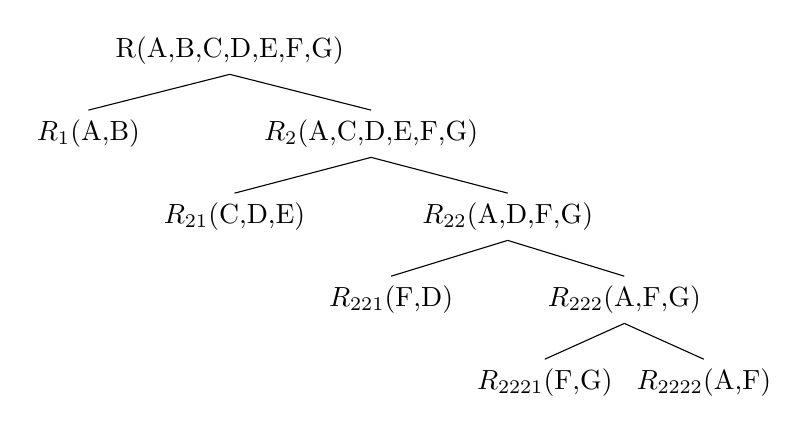
\begin{tikzpicture}[scale=1]
\Tree [.R(A,B,C,D,E,F,G) [.$R_1$(A,B) ][.$R_2$(A,C,D,E,F,G) [.$R_{21}$(C,D,E) ] [.$R_{22}$(A,D,F,G) [.$R_{221}$(F,D) ] [.$R_{222}$(A,F,G) [.$R_{2221}$(F,G) ] [.$R_{2222}$(A,F)  ] ] ] ] ]
\end{tikzpicture}

\end{tcolorbox}

\paragraph{d)} Show that the above decomposition is,\\

\begin{itemize}
    \item Dependency-preserving or not?
    \begin{tcolorbox}
    We can easily deduct that if we join the final relations into one we won't get some certain dependencies back in the global combined relation. For example we see $E \to G$ and $AC \to D$ were in the initial global functional dependency list and we've lost them during the decomposition. Therefore, this decomposition is not dependency-preserving. 
    \end{tcolorbox}
    
    \item Lossless-join or not?
    \begin{tcolorbox}
    We know that any BCNF decomposition is always lossless and here in above we did a BCNF decomposition; but in more detail, we can see that we are able to join final (decomposed) relations using at least one's primary key field and whenever we are able to achieve such joins on all relations we won't have any problems with losing data in the global joined relation. 
    \end{tcolorbox}
\end{itemize}







\newpage
\section{Normalization}

\paragraph{a) } List of all FDs you identified and the corresponding SQL queries to discover them at the end of step 3 above. \\

\begin{tcolorbox}
$A \to E$ \\

SELECT a\\
FROM q5\_table\\ 
GROUP BY a\\
HAVING COUNT(DISTINCT e) $>$ 1 \\
\end{tcolorbox}

\begin{tcolorbox}
$AB \to C$ \\

SELECT a\\
FROM q5\_table\\ 
GROUP BY a, b\\
HAVING COUNT(DISTINCT c) $>$ 1 \\
\end{tcolorbox}

\begin{tcolorbox}
$AB \to E$ \\

SELECT a\\
FROM q5\_table\\ 
GROUP BY a, b\\
HAVING COUNT(DISTINCT e) $>$ 1 \\
\end{tcolorbox}

\begin{tcolorbox}
$AC \to B$ \\

SELECT a\\
FROM q5\_table\\ 
GROUP BY a, c\\
HAVING COUNT(DISTINCT b) $>$ 1 \\
\end{tcolorbox}

\begin{tcolorbox}
$AC \to E$ \\

SELECT a\\
FROM q5\_table\\ 
GROUP BY a, c\\
HAVING COUNT(DISTINCT e) $>$ 1 \\
\end{tcolorbox}

\begin{tcolorbox}
$AD \to E$ \\

SELECT a\\
FROM q5\_table\\ 
GROUP BY a, d\\
HAVING COUNT(DISTINCT e) $>$ 1 \\
\end{tcolorbox}

\begin{tcolorbox}
$BC \to A$ \\

SELECT b\\
FROM q5\_table\\ 
GROUP BY b, c\\
HAVING COUNT(DISTINCT a) $>$ 1 \\
\end{tcolorbox}

\begin{tcolorbox}
$BC \to E$ \\

SELECT b\\
FROM q5\_table\\ 
GROUP BY b, c\\
HAVING COUNT(DISTINCT e) $>$ 1 \\
\end{tcolorbox}

\begin{tcolorbox}
$BE \to A$ \\

SELECT b\\
FROM q5\_table\\ 
GROUP BY b, e\\
HAVING COUNT(DISTINCT a) $>$ 1 \\
\end{tcolorbox}

\begin{tcolorbox}
$BE \to C$ \\

SELECT b\\
FROM q5\_table\\ 
GROUP BY b, e\\
HAVING COUNT(DISTINCT c) $>$ 1 \\
\end{tcolorbox}

\begin{tcolorbox}
$C \to A$ \\

SELECT c\\
FROM q5\_table\\ 
GROUP BY c\\
HAVING COUNT(DISTINCT a) $>$ 1 \\
\end{tcolorbox}

\begin{tcolorbox}
$C \to B$ \\

SELECT c\\
FROM q5\_table\\ 
GROUP BY b\\
HAVING COUNT(DISTINCT b) $>$ 1 \\
\end{tcolorbox}

\begin{tcolorbox}
$C \to E$ \\

SELECT c\\
FROM q5\_table\\ 
GROUP BY e\\
HAVING COUNT(DISTINCT e) $>$ 1 \\
\end{tcolorbox}

\begin{tcolorbox}
$CD \to A$ \\

SELECT c\\
FROM q5\_table\\ 
GROUP BY c, d\\
HAVING COUNT(DISTINCT a) $>$ 1 \\
\end{tcolorbox}

\begin{tcolorbox}
$CD \to B$ \\

SELECT c\\
FROM q5\_table\\ 
GROUP BY c, d\\
HAVING COUNT(DISTINCT b) $>$ 1 \\
\end{tcolorbox}

\begin{tcolorbox}
$CD \to E$ \\

SELECT c\\
FROM q5\_table\\ 
GROUP BY c, d\\
HAVING COUNT(DISTINCT e) $>$ 1 \\
\end{tcolorbox}

\begin{tcolorbox}
$CE \to A$ \\

SELECT c\\
FROM q5\_table\\ 
GROUP BY c, e\\
HAVING COUNT(DISTINCT a) $>$ 1 \\
\end{tcolorbox}

\begin{tcolorbox}
$CD \to B$ \\

SELECT c\\
FROM q5\_table\\ 
GROUP BY c, d\\
HAVING COUNT(DISTINCT b) $>$ 1 \\
\end{tcolorbox}

\begin{tcolorbox}
$DE \to A$ \\

SELECT d\\
FROM q5\_table\\ 
GROUP BY d, e\\
HAVING COUNT(DISTINCT a) $>$ 1 \\
\end{tcolorbox}

\begin{tcolorbox}
$E \to A$ \\

SELECT e\\
FROM q5\_table\\ 
GROUP BY e\\
HAVING COUNT(DISTINCT a) $>$ 1 \\
\end{tcolorbox}

\paragraph{b)} List of all SQL statements to create normalized tables.

\begin{tcolorbox}
CREATE TABLE q5\_AE (\\
	A varchar(20),\\
	E varchar(20),\\
	PRIMARY KEY(A) \\
);\\

CREATE TABLE q5\_ABC ( \\
	A varchar(20),\\
	B varchar(20), \\
	C int, \\
	PRIMARY KEY(C), \\
	FOREIGN KEY(A) REFERENCES q5\_AE(A) \\ 
);\\

CREATE TABLE q5\_CD (\\
	C int, \\
	D int, \\
	PRIMARY KEY(C,D) \\
);
\end{tcolorbox}

\paragraph{c)} List of all SQL statements that load the contents of the tables.

\begin{tcolorbox}
INSERT INTO q5\_AE(a,e) \\
SELECT DISTINCT a,e\\
FROM q5\_table\\

INSERT INTO q5\_ABC(a,b,c) \\
SELECT DISTINCT a,b,c\\
FROM q5\_table\\

INSERT INTO q5\_CD(c,d)\\
SELECT DISTINCT c,d\\
FROM q5\_table
\end{tcolorbox}
\end{document}
